\documentclass{article}
% Author: Luan Leal
% Last update: 2024-12-03

% ----------------------------

% ----------------------------   IMPORTS   ----------------------------
\usepackage{amssymb, amsthm, amsmath, geometry, siunitx, caption, float, graphicx}
\usepackage{enumitem}
\usepackage[utf8]{inputenc}
\usepackage[onehalfspacing]{setspaceenhanced}
\usepackage[brazil]{babel} % Adaptação ao pt-br
\usepackage{hyperref} % Usado para inserir links
\usepackage[capitalize, brazilian, noabbrev]{cleveref} % Referência adaptada ao pt-br
\usepackage{subcaption}
\usepackage{makecell}
\usepackage[num,overcite]{abntex2cite}

% ----------------------------   LAYOUT   ----------------------------
\citebrackets[]
\geometry{a4paper, lmargin=3cm, tmargin=3cm, rmargin=2cm, bmargin=2cm}
\onehalfspacing
%\setlength{\parindent}{45pt}
\sisetup{output-decimal-marker = {,}}

% ----------------------------  THEOREMS  ----------------------------
% -Ambiente de definição
\theoremstyle{definition}
\newtheorem{dfn}{Definição}[section]

% -Ambiente de observação
\theoremstyle{remark}
\newtheorem{obs}{Observação}

% -Ambiente de lema
\theoremstyle{definition}
\newtheorem{lema}{Lema}

% -Ambiente de exemplo
\theoremstyle{definition}
\newtheorem{xp}{Exemplo}[section]

% -Ambiente de proposição
\newtheorem{prop}{Proposição}

% -Ambiente de teorema e demonstração
\theoremstyle{plain}
\newtheorem{thm}{Teorema}
\theoremstyle{remark}
\newtheorem*{dms}{Demonstração}

% -Ambiente de exercício e resolução
\theoremstyle{definition}
\newtheorem{xcs}{Exercício}
\theoremstyle{remark}
\newtheorem*{rsl}{Resolução}

% ----------------------------  COMMANDS  ----------------------------
%\newcommand{\RR}{\mathbb{R}} % \mathbb{R} = \RR
%\newcommand{\ZZ}{\mathbb{Z}} % \mathbb{Z} = \ZZ

\author{Luan Leal (15470820);
; Matheus Queiroz (15479562);\\ Micael Baruch (15578823)}
\title{Relatório 2 --- Determinação do equilíbrio químico} 

\captionsetup{margin=10pt,font=small,labelfont=bf,labelsep=period}

\begin{document}
\maketitle

\section{Equilíbrios envolvidos no experimento}

De maneira simplificada, a reação cujo equilíbrio estamos interessados em acompanhar é a seguinte:
\begin{align*}
    \ce{Fe^{3+}_{aq} + SCN^-_{aq} <-->[{K_1}][{K_2}] {[Fe(SCN)]}^{2+}_{aq}}
\end{align*}

Em que \(K_1 = \cfrac{[{[Fe(SCN)]}^{2+}]}{[Fe^{3+}][SCN^-]} \) e \(K_2 = \cfrac{1}{k_1}\).

No entanto, estamos adicionando \ce{Fe(NO3)3} como fonte de íons ferro e \ce{KSCN} como fonte de íons tiocianato. Neste caso, o real equilíbrio é dado por:

\begin{align*}
    \ce{Fe(NO3)3 + KSCN <-->[{K_3}][{K_4}] Fe^{3+}_{aq} + 3NO3^-_{aq} + SCN^-_{aq} + K^+_{aq} <-->[{k_1}][{k_2}] {[Fe(SCN)]}^{2+}_{aq} + 3NO3^-_{aq} + k^+_{aq}}
\end{align*}

Simultaneamente, pode ocorrer reação entre os íons férricos e a água:

\begin{align*}
    \ce{Fe^{3+}_{aq} + 2H2O_l <-->[{K_5}][{K_6}] {(Fe(OH))}^{2+}_{aq} + H3O^+_{aq}}
\end{align*}

Ainda assim, como \(K_3\) é muito maior que \(K_4\) pode-se tomar como negligenciável a etapa de ionização. Quanto à reação com íons férricos e água, para isto é adicionado ácido nítrico à solução, o ácido nítrico é forte e é completamente ionizado na água, resultando na formação excessiva de \ce{H3O+}  que resulta na não reação de água com \(\ce{Fe^{3+}}\) mantendo sua disponibilidade para a reação de interesse.   

\section{Outras propriedades para determinar as constantes de equilíbrio}

\section{Determine a curva de calibração do \ce{{[Fe(SCN)]}^{2+}}}
Para determinação da curva de calibração foram feitas soluções ricas em \ce{FeNO3} em comparação ao \ce{KSCN}. O objetivo disto é que desta forma há excesso de íons férricos de tal forma que toda concentração disponível de \ce{KSCN} reage para formar \ce{Fe(SCN)}. Ou seja, a concentração final de \ce{Fe(SCN)} é igual à concentração inicial de \ce{KSCN}. Tirando a média dos dados dos diferentes grupos da sala obtivemos a curva de calibração descrita na \cref{curvaPadrao}

\begin{figure}[H]
    \centering
    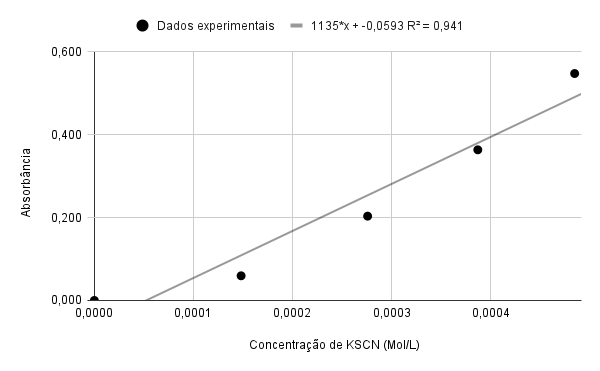
\includegraphics[width=.5\linewidth]{fig/curvaPadrao}
    \caption{Curva de calibração do \ce{Fe(SCN)} obtida pela média dos valores experimentais dos grupos da sala. A equação de reta que descreve a curva está apresentada na parte superior da figura.}\label{curvaPadrao}
\end{figure}

\section{Determine a constante de formação do \ce{{[Fe(SCN)]}^{2+}}. Compare com um valor encontrado na literatura e calcule o erro absoluto e o erro relativo}

\section{Que fatores experimentais desviaram as constantes obtidas? Por quê?}

    \bibliographystyle{plain}
    \bibliography{bibliography}

\end{document}
